In this section, we present and analyze the results obtained from the experiments conducted on the methods introduced in the previous chapters. For each macro-category, two algorithmic approaches were implemented. The analysis is divided into two phases: first, the main parameters are fine-tuned (when applicable), and then the best-performing configurations within each category are compared.

\section{Methodology}

Each group of algorithms is analyzed independently, following a consistent methodology. Three main parameters are considered throughout the experiments:
\begin{itemize}
    \item \textbf{Number of nodes:} This varies depending on the method's nature (e.g., fewer nodes for exact methods, more for heuristics and metaheuristics).
    \item \textbf{Time limit:} A fixed time budget is set for all experiments to ensure comparability.
    \item \textbf{Number of runs:} Each configuration is tested on 20 randomly generated instances to ensure statistical significance.
\end{itemize}

Specifically, the following settings were adopted:
\begin{itemize}
    \item \textbf{Heuristics:} 1000-node instances, 120-second time limit.
    \item \textbf{Metaheuristics:} 1000-node instances, 120-second time limit.
    \item \textbf{Exact methods:} 300-node instances, 120-second time limit.
    \item \textbf{Matheuristics:} 1000-node instances, 180-second time limit.
\end{itemize}

Each test was repeated on 20 instances, initialized with distinct random seeds. To enable rigorous comparisons, we rely on \textbf{performance profiles}, a graphical benchmarking tool that allows us to assess and visualize the relative efficiency of different algorithms across a set of problem instances~\cite{dolan2002performance}.

\subsection{Instance Generation}

The TSP instances used in our experiments are generated randomly. Each instance consists of a set of points placed on a 2D grid $[0, 10\,000] \times [0, 10\,000]$, with coordinates sampled from an independent and identically distributed model. The cost matrix for each instance is computed using the Euclidean distance between points, optionally rounded according to the \emph{ATT} formula from TSPLIB~\cite{reinelt1995tsplib}.

\subsection{Experimental Setup}

The exact and matheuristic methods were solved using \textbf{IBM ILOG CPLEX 22.1.2}~\cite{cplex2023}, interfaced via its C API. Greedy and heuristic algorithms were implemented in C for performance reasons, while Python was used for result visualization and data processing.

To ensure comparability, all algorithms within the same category were executed sequentially on the same hardware. However, different classes of methods were executed on different machines, as detailed below:

\begin{center}
\begin{tabular}{ c | c | c }
  \textbf{Processor} & \textbf{RAM} & \textbf{Algorithms Executed} \\
  \hline
  Intel Core i7-10510U & 16 GB & Exact, Matheuristic \\
  Intel Core i5-8265U  & 16 GB & Greedy, Heuristic \\
\end{tabular}
\end{center}

\subsection{Performance Profiles}

To compare algorithm performance across a common set of instances, we used performance profiles. These were generated using a Python script developed by Professor Domenico Salvagnin. The script processes a CSV file containing the results of each algorithm on each instance and compares the performance to the best value achieved on that instance.

This approach enables the construction of plots that show, for each algorithm, the proportion of instances for which its performance is within a given factor of the best. For heuristic and metaheuristic methods, the comparison is based on the objective value of the best solution found; for exact methods, it is based on the time required to find the optimal solution.

\section{Parameters tuning}

\subsection{Nearest Neighbor - Greedy}
\label{ssec:nn-tuning}

In the case of Nearest Neighbor method we don't have any parameters to tune, but we can analyze if the Two-Opt step is beneficial or not. It is intuitive from the definion presented in section \ref{sec:2opt} that the 2-opt step is always beneficial, as it can only improve the quality of the tour. For completeness, we report the performance profiles of the Nearest Neighbor method with and without the 2-opt step in Figure~\ref{fig:nn-profiles}.

\begin{figure}[H]
  \centering
  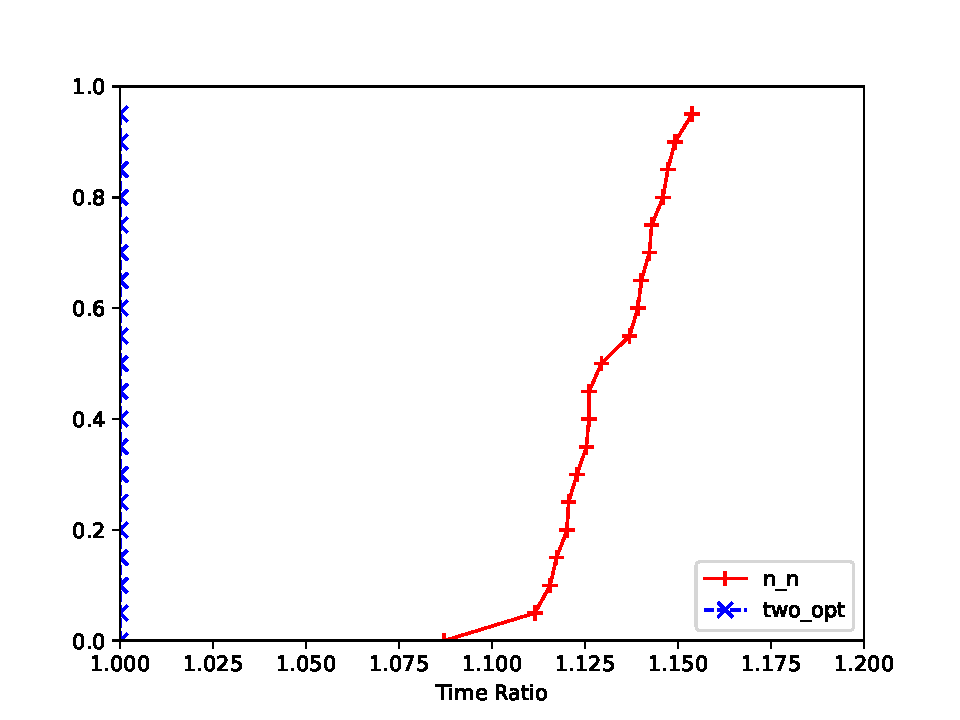
\includegraphics[width=0.8\textwidth]{greedy_profiles.pdf}
  \caption{Performance profiles for the Greedy method.}
  \label{fig:nn-profiles}
\end{figure}

\subsection{Tabu Search}
\label{ssec:tabu-tuning}
As discussed in Section~\ref{sec:tabu}, Tabu Search relies on a short-term memory of forbidden moves, whose size is governed by the base tenure \(T\).  In many works one selects a single ratio \(\alpha\) and sets \(T=\frac{N_{\mathrm{nodes}}}{\alpha}\), but this hides the fact that the method can be tuned more flexibly by independently controlling the dynamic bounds \(T_{\min}\) and \(T_{\max}\).

In our implementation we therefore allow the user to specify all parameters directly, allowing also for setting the cutoff for forced diversification, \(N_{\mathrm{ni}}\). Conceptually, however, it is still suggested to leverage the ratio \(\alpha\) to derive the base tenure \(T\).

Table~\ref{tab:tabu-configs} reports the eight configurations where we tried to span as many different search behaviors as possible.

\begin{table}[H]
  \centering
  \caption{Tabu search configurations}
  \label{tab:tabu-configs}
  \resizebox{\textwidth}{!}{%
  \begin{tabular}{|c|c|c|c|l|}
    \hline
    \textbf{$T$} & \textbf{$T_{\min}$} & \textbf{$T_{\max}$} & \textbf{$N_{\mathrm{ni}}$} & \textbf{Description} \\ 
    \hline
    227 & 10 & 227 & 500 & Good balance, but no expansion beyond the initial tenure. \\
    250 & 10  & 375  & 500  & Moderate diversification via expanded max tenure. \\ 
    208 & 5   & 416  & 1000 & Broad tenure span allows prolonged exploration before reset. \\ 
    278 & 20  & 278  & 250  & Fixed high tenure intensifies local moves with quick shake-up. \\ 
    167 & 10  & 167  & 500  & Small tenure forces rapid neighborhood changes. \\ 
    333 & 10  & 500  & 500  & Max tenure scaled to problem size supports deeper history. \\ 
    100 & 5   & 500  & 200  & Very short base tenure and low cutoff for intense shaking. \\ 
    400 & 50  & 400  & 2000 & Large tenure and high cutoff delay diversification for global search. \\ 
    \hline
  \end{tabular}%
  }
\end{table}

Results highlight that configurations with a large base tenure and a wide dynamic span tend to converge more quickly to high-quality incumbents. In particular:
\begin{itemize}
  \item \emph{High base tenure}: retaining a long short-term memory before forcing diversification produces the best overall performance, by exploiting promising regions.
  \item \emph{Wide dynamic window}: allowing the tabu tenure to expand and contract over a large interval helps escape local optima when progress stalls.
  \item \emph{Medium settings}: a moderate base tenure with a moderately sized dynamic range provides a reasonable trade-off between intensification and diversification, but does not match the extremes.
  \item \emph{Small or rigid tenure}: very short or fixed tabu lists lead to slower discovery of good solutions and a greater risk of stagnation.
\end{itemize}

\begin{figure}[H]
  \centering
  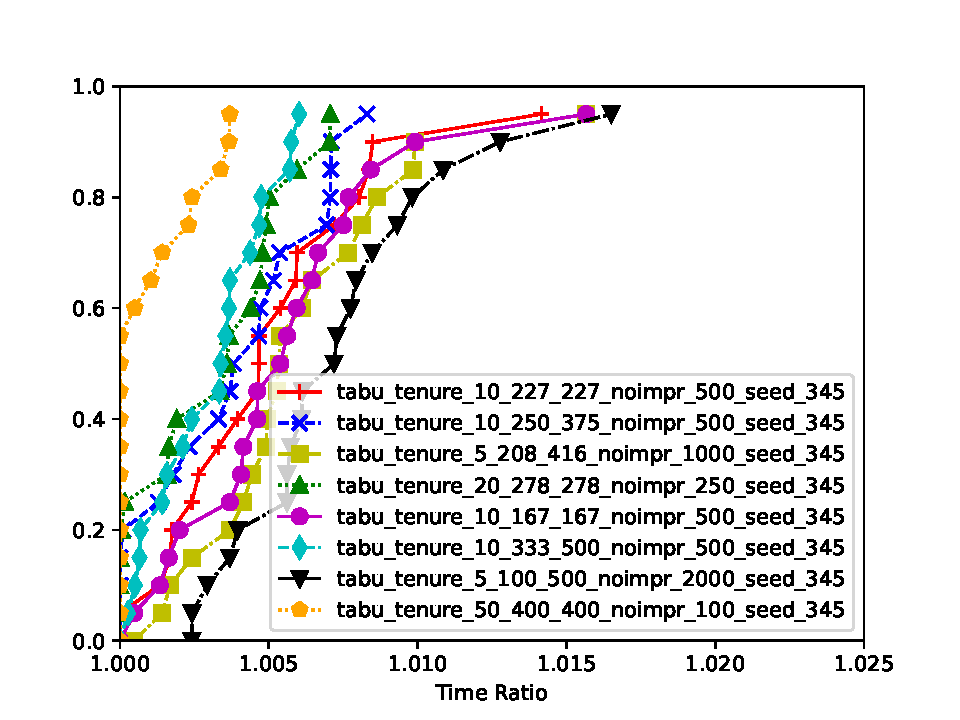
\includegraphics[width=0.8\textwidth]{tabu_profiles.pdf}
  \caption{Performance profiles for the Tabu Search configurations.}
  \label{fig:tabu-profiles}
\end{figure}

\subsection{Varable Neighborhood Search}
\label{ssec:vns-tuning}

To find the best configuration for the VNS algorithm, we focused on the parameters that control the number of 3-opt “kicks” applied per iteration. We let the user specify a fixed number of kicks \(J\) or an adaptive scheme that draws a number of kicks uniformly from a range \([k_{\min},k_{\max}]\), scaled by a learning rate \(\lambda\). Table~\ref{tab:vns-configs} summarizes the settings we evaluated:

\begin{table}[H]
  \centering
  \caption{VNS configurations}
  \label{tab:vns-configs}
  \resizebox{\textwidth}{!}{%
  \begin{tabular}{|c|c|c|c|c|l|}
    \hline
    \textbf{ID} & \(\boldsymbol{k_{\min}}\) & \(\boldsymbol{k_{\max}}\) & \(\boldsymbol{\lambda}\) & \(\boldsymbol{J}\) & \textbf{Description} \\ 
    \hline
    1 & 2   & 4   & 1.00 & -  & Balanced adaptive kicks. \\ 
    2 & 1   & 5   & 1.00 & -  & Wide range for broader exploration. \\ 
    3 & 2   & 6   & 1.00 & -  & Extended range for more diversification. \\ 
    4 & 1   & 10  & 1.00 & -  & Very wide span, high diversification. \\ 
    5 & 2   & 4   & 0.50 & -  & Conservative kicks (half learning rate). \\ 
    8 & 2   & 4   & 2.00 & -  & Aggressive kicks (double learning rate). \\ 
    6 & -   & -   & -    & 3  & Fixed few kicks per iteration. \\ 
    7 & -   & -   & -    & 10 & Fixed many kicks, conservative scale. \\ 
    \hline
  \end{tabular}%
  }
\end{table}

Results presented in Figure \ref{fig:vns-profiles} suggest that a fixed number of kicks per iterations is more effective than adaptive schemes. In particular, the more kicks are applied the better the results, with the with the configuration applying 10 kicks outperforming all others. Anyways, the adaptive schemes still perform reasonably well, especially when the range of kicks is wide enough to allow for sufficient exploration.

\begin{figure}[H]
  \centering
  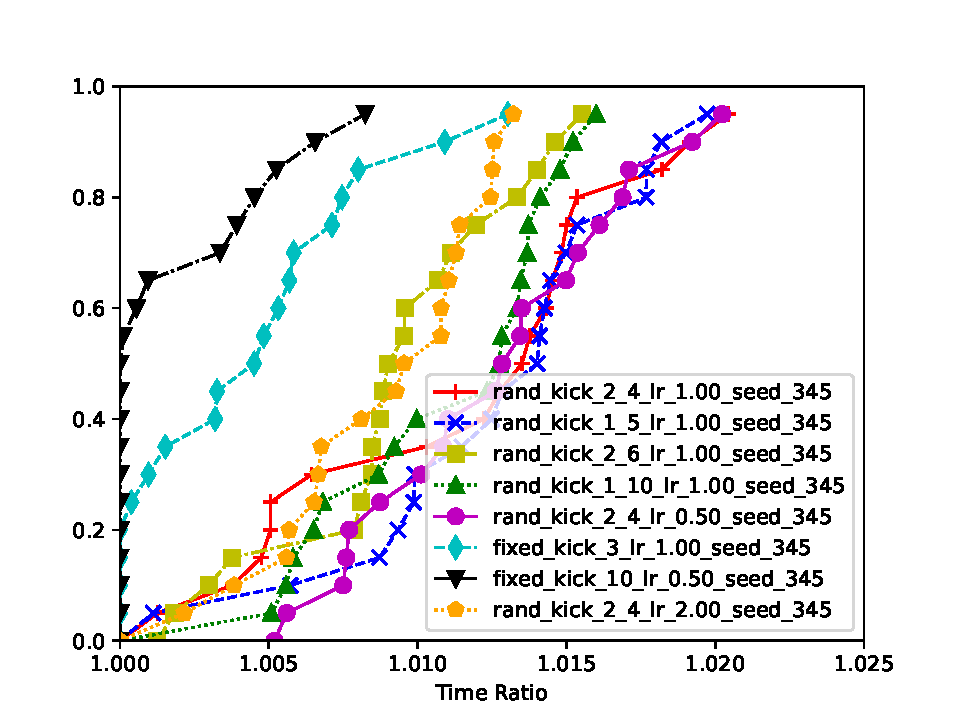
\includegraphics[width=0.8\textwidth]{vns_profiles.pdf}
  \caption{Performance profiles for the VNS configurations.}
  \label{fig:vns-profiles}
\end{figure}

\subsection{Hard Fixing}
\label{ssec:hard-fixing}

The Hard Fixing method depends on two key parameters: the proportion of edges to fix and the local time limit allocated to CPLEX for solving each subproblem. In preliminary experiments on 1,000-node instances with a global time limit of 180 s, we observed that fixing fewer than 50\% of the arcs provided no appreciable benefit, as the CPLEX time limits were too restrictive. Consequently, we concentrated our study on fixing between 60\% and 80\% of the arcs. We also varied the local time limit to strike a balance between the number of iterations executed per run and the time CPLEX requires to solve each resulting subgraph, all proportionally scaled to the overall 180 seconds budget.

Figure \ref{fig:hf-profiles-general} shows that fixing 70\% of the arcs yields a more robust performance than the 60\% configurations, while variations in the local time limit have only a marginal impact on the shape of the profile. To fine-tune the method, we therefore fixed the local time limit at 30 seconds, identified as the most robust among those tested, and extended our comparison to include the 80\% fixing level.

\begin{figure}[H]
  \centering
  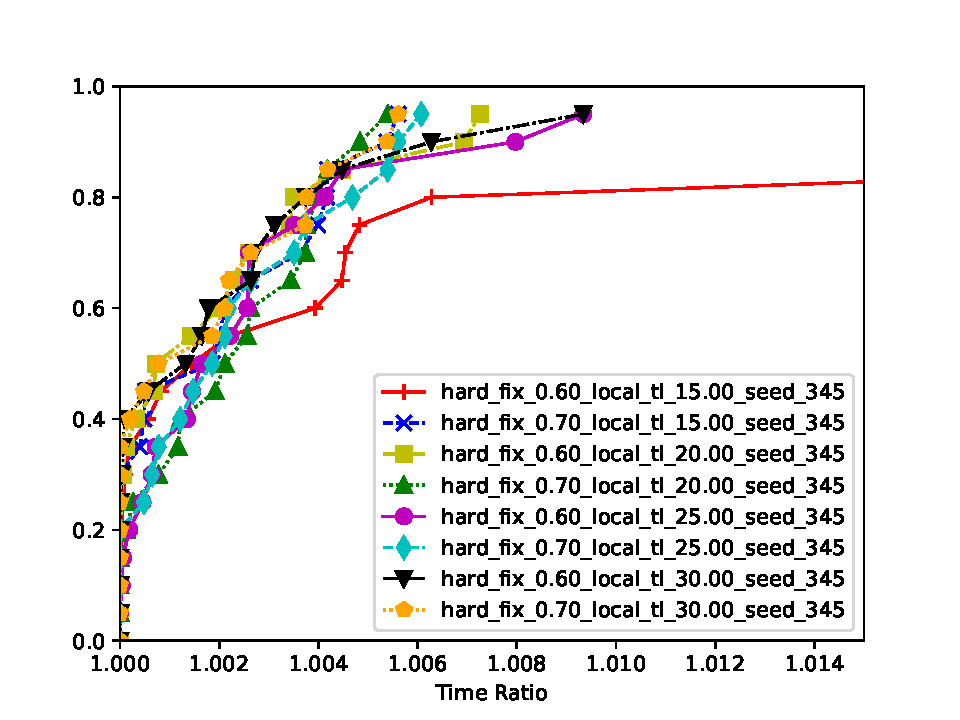
\includegraphics[width=0.8\textwidth]{hf_profiles.pdf}
  \caption{Performance profiles for Hard Fixing with varying fixing ratios and local time limits.}
  \label{fig:hf-profiles-general}
\end{figure}

Figure \ref{fig:hf-profiles-30sec} compares the three fixing ratios with the local time limit held constant at 30 second. It confirms that constraining the arcs too tightly degrades performance, whereas the 70\% fixing level still achieves the highest coverage across those tested.

\begin{figure}[H]
  \centering
  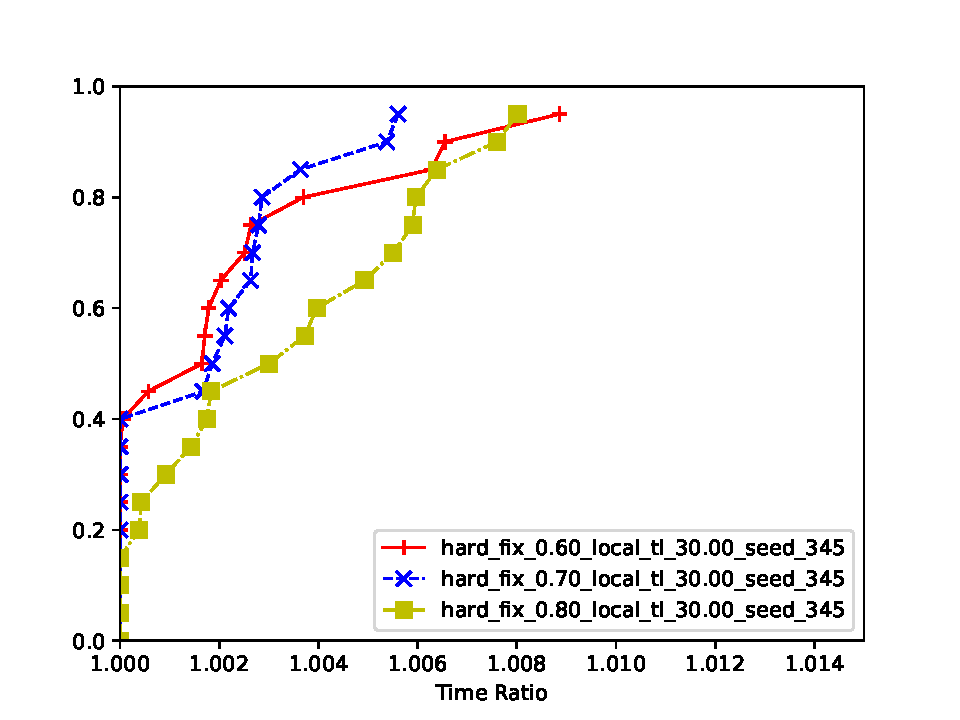
\includegraphics[width=0.8\textwidth]{hf_profiles2.pdf}
  \caption{Performance profiles for Hard Fixing with a fixed 30 s local time limit.}
  \label{fig:hf-profiles-30sec}
\end{figure}

Overall, the combination of fixing 70\% of the arcs and allowing a 30 sec local solve time delivers the best trade-off between solution quality and robustness.

\subsection{Local Branching}
\label{ssec:local-branch}

We evaluate the impact of two tuning parameters on the Local Branching heuristic: the initial neighborhood size \(K\) and the incremental step by which \(K\) is adjusted at each iteration. Figure~\ref{fig:lb-profiles} presents performance profiles comparing various \((K,\text{step})\) configurations under a fixed time budget.

\begin{figure}[H]
  \centering
  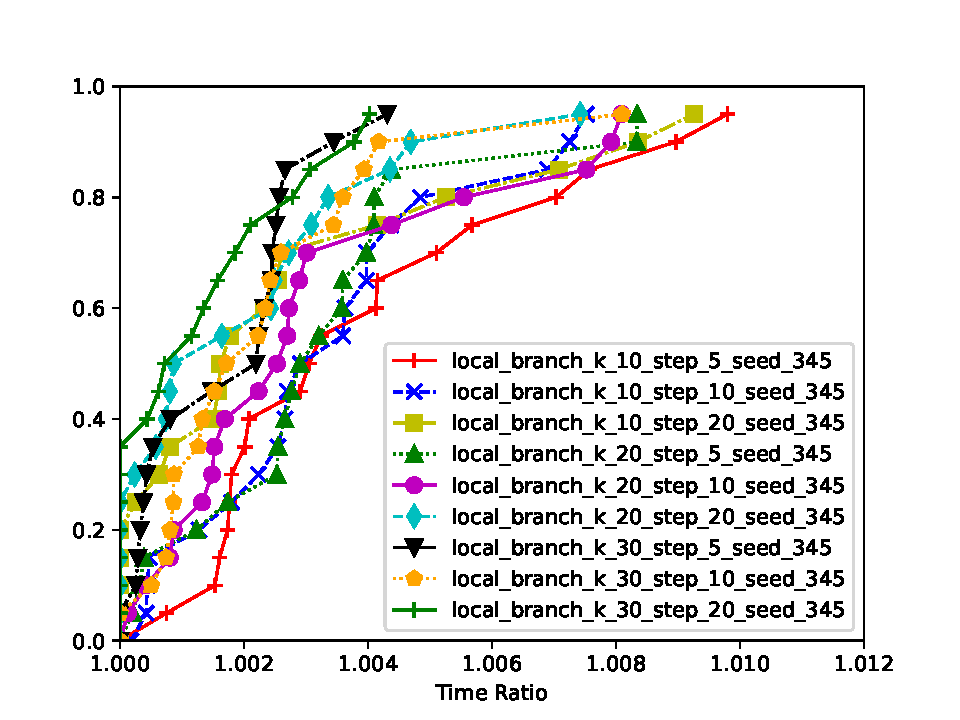
\includegraphics[width=0.8\textwidth]{lb_profiles.pdf}
  \caption{Performance profiles for Local Branching across different choices of \(K\) and step size.}
  \label{fig:lb-profiles}
\end{figure}

The results show that larger neighborhoods yield more consistent improvements: configurations with \(K=30\) uniformly outperform those with \(K=20\) and \(K=10\). Likewise, a step size of 20 delivers the fastest early gains, although its marginal benefit diminishes over longer runs. Overall, the combination \(K=30\) and \(\text{step}=20\) achieves the best final costs under our time constraint.  

\section{Methods comparison}

\subsection{Best Heuristic - Full time limit}

After tuning the parameters of the Tabu Search and VNS algorithms we now compare their performance to determine the best heuristic for solving the TSP. We assume that the experiments performed during the parameters tuning phase cover a wide range of search behaviors and thus considering the four best configurations of each method is sufficient to draw conclusions on the overall performance of the two methods.

\begin{figure}[h]
  \centering
  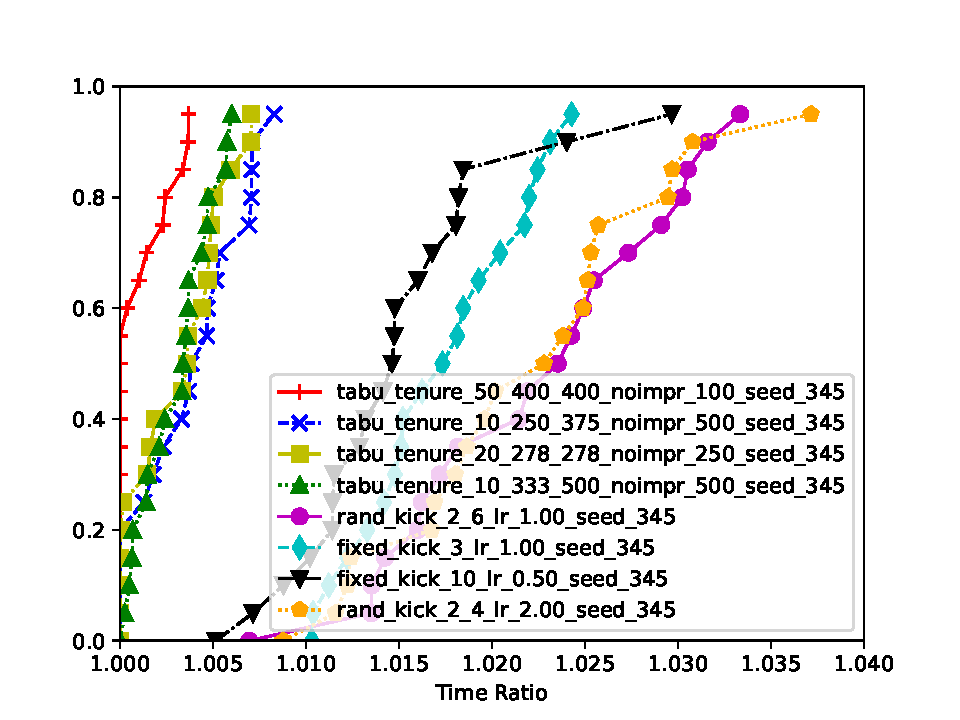
\includegraphics[width=0.8\textwidth]{best_heuristic_profiles.pdf}
  \caption{Performance profiles to compare VNS and Tabu Search.}
  \label{fig:best-heuristic-profiles}
\end{figure}

Looking at Figure \ref{fig:best-heuristic-profiles} there is no doubt on the superiority of the Tabu Search algorithm, the method configurations used in the comparison cover different search behaviours and all outperform the VNS configurations.

One more interesting comparison is to check how an approach as simple as the Nearest Neighbor with 2-opt compares to the best heuristic. The results are shown in Figure \ref{fig:nn-vs-best-heuristic} and clearly show that the complicated and time-demanding search performed by Tabu is justifide by the quality of the solutions found, which is significantly better.

\begin{figure}[H]
  \centering
  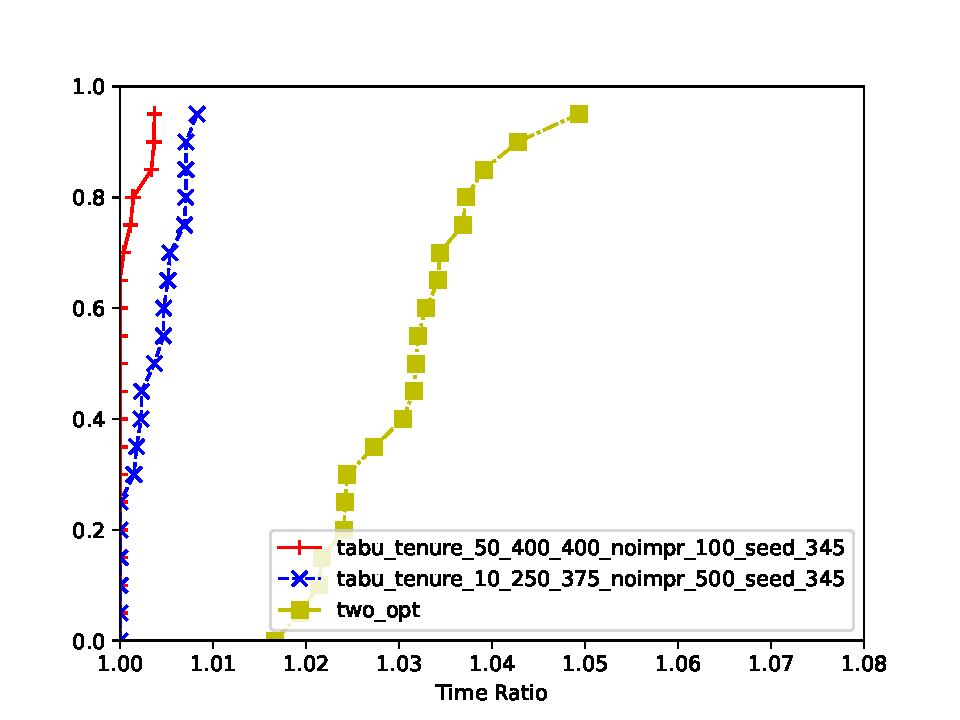
\includegraphics[width=0.8\textwidth]{nn_tabu_profiles.pdf}
  \caption{Tabu Search compared to Nearest Neighbor with 2-opt.}
  \label{fig:nn-vs-best-heuristic}
\end{figure}

\subsection{Best Heuristic - Short Time Budget}
\label{ssec:short-heuristic}
All CPLEX-based exact methods are initialized with a heuristic solution obtained by allocating 10\% of the total time limit to the heuristic. To identify the most effective warm-start configuration, we therefore evaluate our top Tabu Search settings using a reduced time budget of 12 seconds. The best-performing configuration from this experiment will be used to warm-start the exact methods, which are compared in the next chapter. Since the instances of exact methods will be smaller, we are now searching for percentages of the number of nodes to set the tenure size, rather than absolute values.

From Figure \ref{fig:fast-heuristic} we can see that the best-performing configuration now is the one with a tenure size of around 28\% of the number of nodes and a minimum size of 2\%. This is a sigificant difference from the previous experiments, where the bigger tenure size was the best, this is likely due to the fact that with a short time limit the algorithm needs to explore more and thus a smaller tenure size allows for more diversification.

\begin{figure}[H]
  \centering
  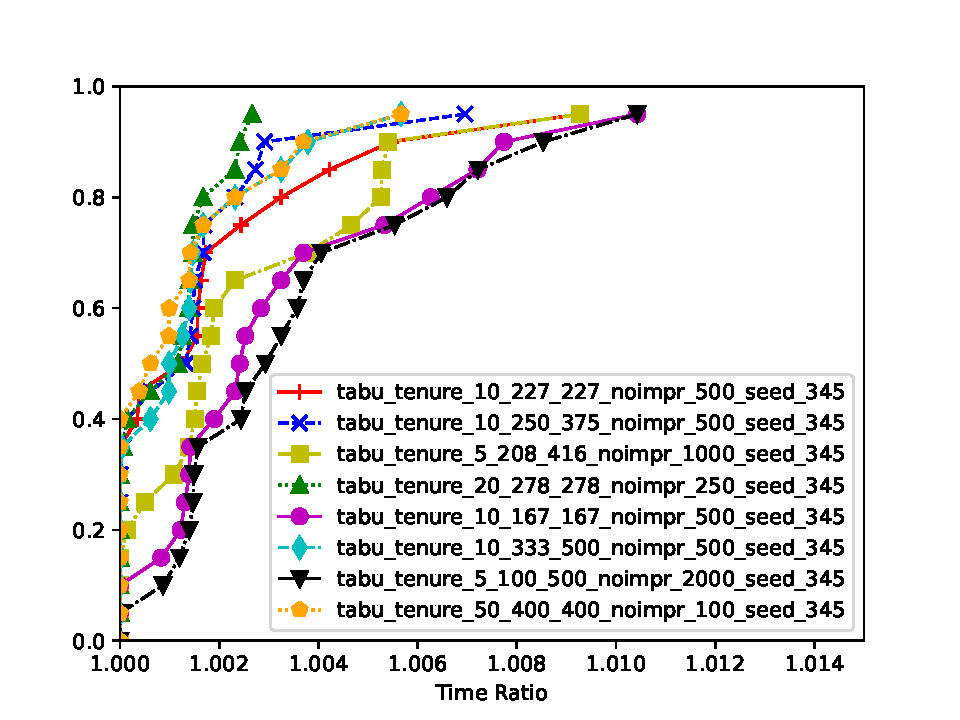
\includegraphics[width=0.8\textwidth]{fast_heuristic_profiles.pdf}
  \caption{Tabu Search performance profiles under a 12-second time limit.}
  \label{fig:fast-heuristic}
\end{figure}

\subsection{Best Exact Method}

This section compares the Exact Methods introduced in Chapter \ref{chap:exact-methods}. While these methods do not involve any fine-tuning, we still explore variations in their configurations to evaluate performance differences. Specifically, we examine three different approaches for initializing the solver:

\begin{itemize}
\item \textbf{No Warm Start}: In this baseline approach, CPLEX performs the optimization from scratch without any preprocessing or initial solution.
\item \textbf{Heuristic Warm Start}: As discussed in Section \ref{ssec:short-heuristic}, we identified the best configuration for a time-limited heuristic. The solution obtained from this heuristic is used as the starting point for the exact solver.
\item \textbf{Two-Opt Warm Start}: We observed that a simple greedy solution refined with the two-opt technique yields a reasonable solution in under one second. Although typically worse than the heuristic solution, we aim to test whether this quick-start approach can help the exact method reach optimality faster.
\end{itemize}

\begin{figure}[H]
  \centering
  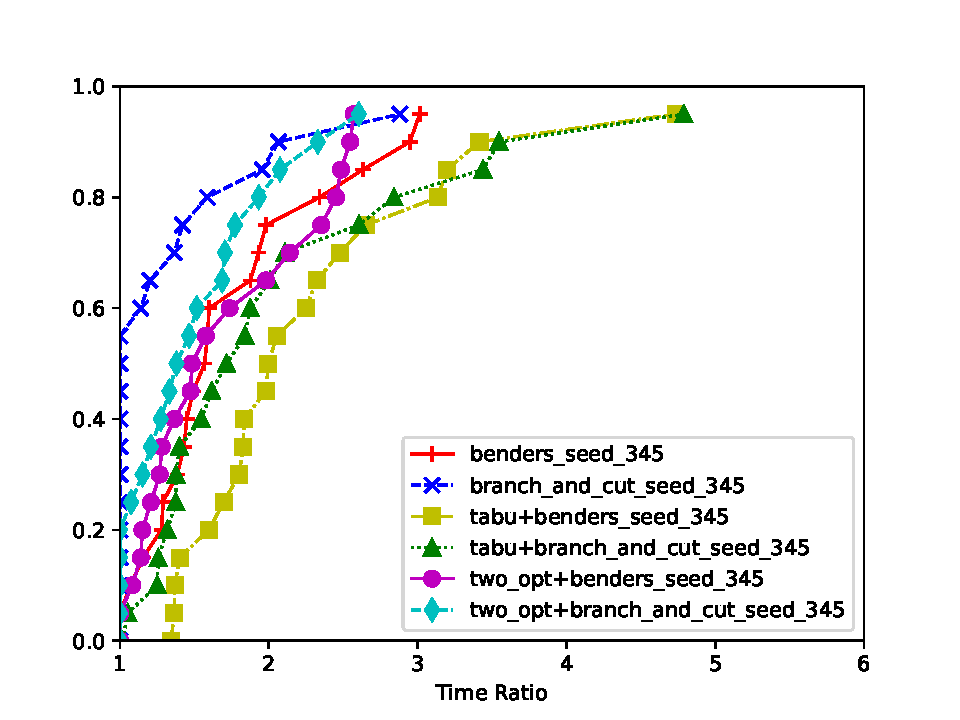
\includegraphics[width=0.8\textwidth]{exact_profiles_new.pdf}
  \caption{Exact Methods performance profiles.}
  \label{fig:exact}
\end{figure}

Figure~\ref{fig:exact} shows the performance profiles of the exact solver under different initialization strategies. The standard \textbf{Branch-and-Cut} method performs best overall, solving the highest fraction of instances quickly and consistently across all time ratios. Its variant initialized with a \textbf{Two-Opt} solution performs comparably in the long run but lags slightly in early time windows, indicating that the warm start introduces some initial overhead without clear benefits in this setting.

In contrast, \textbf{Two-Opt} offers a more tangible advantage when paired with \textbf{Benders}. While it initially solves slightly fewer instances than plain Benders, it eventually overtakes it, demonstrating that lightweight local search can improve convergence over time.

Warm starts based on the \textbf{Tabu} heuristic consistently underperform. Whether combined with Benders or Branch-and-Cut, these configurations solve fewer instances across all time ratios, likely due to the higher overhead of Tabu not being compensated by solution quality.

Overall, default configurations—particularly Branch-and-Cut—remain highly effective. Lightweight warm starts like Two-Opt may be beneficial, especially for Benders, but more expensive ones like Tabu tend to degrade performance.

\subsection{Best Matheuristic}
\label{ssec:best-matheu}

In this section we compare the matheuristic methods from Chapter~\ref{chap:matheuristics} after parameter tuning. Figure~\ref{fig:matheu} clearly shows that Hard Fixing clearly outperforms Local Branching.

\begin{figure}[H]
  \centering
  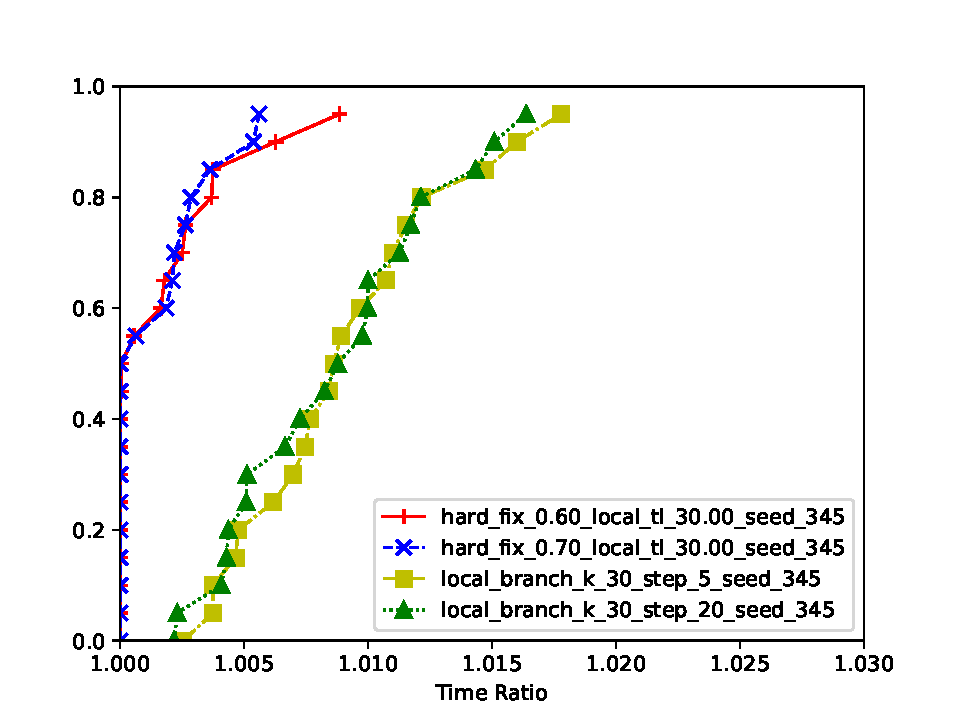
\includegraphics[width=0.8\textwidth]{matheu.pdf}
  \caption{Performance profiles for the tuned matheuristics.}
  \label{fig:matheu}
\end{figure}

These results can be attributed to Hard Fixing's strategy of locking in high-quality variable assignments, which focuses the solver on the most promising regions of the search space and produces strong incumbents much faster than the incremental neighborhood adjustments of Local Branching.  
